\documentclass[letter, 11pt]{article}
\usepackage[utf8]{inputenc}
\usepackage[english]{babel}
\usepackage{amsfonts}
\usepackage{amsmath}
\usepackage[dvips]{graphicx}
\usepackage{url}
\usepackage[top=3cm,bottom=3cm,left=3.5cm,right=3.5cm,footskip=1.5cm,headheight=1.5cm,headsep=.5cm,textheight=3cm]{geometry}
\usepackage{listings}
\usepackage{color}
\usepackage{fancyvrb}
\usepackage{fancyhdr}
\usepackage{enumerate}
\usepackage{amssymb}
\usepackage{multirow}
%% to use the warpfigure capability
\usepackage{wrapfig} 

%%%%%%%%%%%%%%%%%%%%%%
%Estilo del documento%
%%%%%%%%%%%%%%%%%%%%%%
\pagestyle{fancyplain}

%%%%%%%%%%%%%%%%%%%%%%%%%%%%%%%%%%%%%%%%%%%
%Fancyheadings. Top y Bottom del documento%
%%%%%%%%%%%%%%%%%%%%%%%%%%%%%%%%%%%%%%%%%%%
% Recuerde que en este documento la portada del documento no posee
% numeracion, pero de igual manera llamaremos a esa primera pagina la numero
% 1, y la que viene la dos. Esto es para tener una idea de las que
% llamaremos pares e impares
\lhead{} %Parte superior izquierda
\rhead{\bf \it UTFSM, Casa Central} %Parte superior derecha
\lfoot{JSCO} %Parte inferior izquierda.
\cfoot{} %Parte inferior central
\rfoot{\bf \it Page \thepage} %Parte inferior derecha
\renewcommand{\footrulewidth}{0.4pt} %Linea de separacion inferior


\begin{document}
%%%%%%%%%%%%%%%%%%%%%%%%%%%
% Tema de las referencias %
\bibliographystyle{unsrt}
%%%%%%%%%%%%%%%%%%%%%%%%%%

%%%%%%%%%%%%%%%%%%%%%%%%%%
%Definicion de la portada%
%%%%%%%%%%%%%%%%%%%%%%%%%%
\begin{titlepage}
    \begin{center}
	\begin{tabular}{ccc}
	    
\includegraphics[width=3cm]{img/utfsm}
	    & 
	    \hspace{-0.2cm}
	    \begin{tabular}{c}
		Universidad T\'ecnica Federico Santa Mar\'ia \\ \hline
		\vspace{0.2cm}
		Departamento de Inform\'atica\\
		\vspace{1.2cm}
	    \end{tabular}
	    \hspace{0.2cm}
	    &
            
\includegraphics[width=2cm]{img/di}
	\end{tabular}

	\vspace{1cm}
	%Titulo del Documento
	\begin{tabular}{c}
		\Huge{\sc{Testing, Detection and Possible}}\\\\
		\Huge{\sc{Solutions for the Bufferbloat}}\\\\
		\Huge{\sc{Phenomenon on Networks.}}\\\\
		\Large{\sc{State of Art}}\\\\
	\end{tabular}

    	\vspace{2cm}
	\Large{\sc{JUAN S. CATALAN OLMOS}}\\
	\vspace{2cm}
	\large{Definici\'on de Tema de Memoria}\\
	\large{para optar al T\'itulo de:}\\
	\large{INGENIERO CIVIL INFORMATICO}\\
	\vspace{2cm}
         	\normalsize{Profesor Gu\'ia: Horst H. von Brand Skopnik}\\
         	\normalsize{Profesor Coreferente: Ra\'ul Monge Anwandter}\\
	%Fecha
    
    \vspace{2cm}
    \normalsize{\sc{\today}}\\
    \normalsize{\sc{Valpara\'iso, Chile}}\\
    \end{center}
\end{titlepage}


\newpage

%section Intro
\section{Introduction}

According to the reports published by SUBTEL to the first half of 2013,
\textit{12.8} per 100 inhabitants have access to broadband
Internet\cite{OCDE}.  This steady growth is largely due to the emergence of
new applications such as streaming video and music, online gaming and
bandwidth intensive applications.

Not long ago, the links had a much more limited bandwidth than they have
today. With the evolution of electronics and telecommunications,
speeds have increased dramatically. With the current level of data flowing
through the network, it is important to control congestion that
might occur. This is one of the tasks of the routers.

It is important to remember that the traffic in a network is inherently
bursty, the role of the buffers in the router is to smooth the flow of
traffic. Without any buffering, to allocate the bandwidth evenly would be
impossible. But there are some problems with current algorithms; they use
tail-drop based queue management that has two big drawbacks: 1.- lockout 2.-
full queue that impact with a high queue delay.

Current low hardware prices make memory cheap,
and with the ``more is better'' mentality have led to the inflation and
proliferation of buffers everywhere\cite{NicholsJacobsonCQD}. When a router
joins two networks with different bandwidths, each packet is squeezed down in
bandwidth, it must stretch out in time since its size stays constant. When
the queue starts to grow, more and more memory is deployed leading to
massive standing queues. It turns out that this is a recipe for Bufferbloat.
Evidence of Bufferbloat has been accumulating over the past decade, but its
existence has not yet become a widespread cause for concern.

Bufferbloat creates large delays but no improvement in throughput. It is not a
phenomenon treated by queueing or traffic theory, which unfortunately results
in it being almost universally misclassified as congestion. The \textit{\gls{Bufferbloat}}
problem, making the window match the pipe size, is hard to address. Window
sizes are chosen by senders while queues manifest at bottleneck gateways.


As mentioned by Jim Gettys and Kathleen Nichols;
\textit{Today's networks are suffering from unnecessary latency and poor
system performance. The culprit is Bufferbloat, the existence of excessively
large and frequently full buffers inside the network. Large buffers have been
inserted all over the Internet without sufficient thought or testing. They
damage or defeat the fundamental congestion-avoidance algorithms of the
Internet's most common transport protocol. Long delays from Bufferbloat are
frequently attributed incorrectly to network congestion, and this
misinterpretation of the problem leads to the wrong solutions being
proposed}\cite{GettysNichols}.

The objective of this thesis work is checking the effects of
Bufferbloat phenomenon, test the impact that it has on different networks
and to propose solutions. To accomplish this, it first requires to
address the following general objectives:

\begin{itemize}
	\item To define the \textit{Bufferbloat} phenomenon, and explain the impact that it could have on latency and \gls{Throughput}(related to \gls{System Throughput}) in Internet.
	\item To detect its presence by measurements of the latency and throughput in a TCP/IP Network.
	\item To propose solutions in the implementation of a network where the existence of excessively large and frequently buffers are detected
\end{itemize}

In order to archive theses objectives:

\begin{itemize}
\item Develop appropriate tests to be able to prove the existence of \textit{Bufferbloat}
\item To test and differentiate the possible causes of the excessive latency and throughput reduction in a TCP/IP LAN and check how much is generated by \textit{Bufferbloat} or by a miss-configuration
\item To propose configuration of the TCP parameters in a Linux based machine or an algorithm that can help to minimize the phenomenon.
\end{itemize}

Chapter 2 explains the basis on which TCP was developed and
the fundamentals for the current operation of the Internet. The conservation
principle upon which all communication protocols are based will be explained.
It also describes each of the four phases of TCP.

In Chapter 3 we will review one of the most important components for the
communication and the main place where the packages are stored: the Routers.
We will analyze how their queues have a destructive size for
communication, why they are stalled at full capacity and cause excessive
latency. We also consider how to define the appropriate buffer size in a router.

Chapter 4 presented a technique developed to deal more efficiently with
actively congestion that could generate not only on endpoints but also on
routers. This technique is Active queue management (AQM). How the first
algorithms, such as RED and BLUE, were implemented and mention
CODEL which aims to solve the Bufferbloat phenomenon; This failures points,
in both TCP and AQM, are synthesized and analyze. All this will be presented in
Chapter 5.

Chapter 6 aims to define the methodology and tools that will be used to
perform each of the tests to determine the existence and the effects of
Bufferbloat. Each test is defined by its propose starting with some general
tests to check the behavior and sanity of the network and moving to a more
user-related effects of the Bufferbloat. All the tools used are Open Source
projects available for all commercial operative systems. In Chapter 7 the
results of all tests are presented, leading to the conclusions of this work in
chapter 8.


%end intro
%section Foundation
\section{The Bufferbloat Foundations}
\subsection{The TCP Protocol \cite{rfc793}\cite{rfc2001}}
%http://www.linktionary.com/c/congestion.html
%http://condor.depaul.edu/jkristof/technotes/congestion.pdf 

The Transport Control Protocol or TCP is main transport protocol of the
internet, providing reliable host to host communication over unreliable
transport media\cite{rfc793}. The advantages of its connectionless design,
flexibility and robustness provides reliable, ordered delivery of a stream of
bytes from a program on one computer to another program on another computer,
but for that, the cost are: the needed of careful design so it provides a good
service under heavy loads. Many modifications has been done since it was
originally defined in 1981.

The root idea of any algorithm related to transport connections must be based
into the ``\textit{packet conservation principle}". This principle claims:

\begin{defn}
A new packet isn't put into the network until an old packet leaves.
\end{defn}


\subsubsection{Slow-Strart Algorithm\cite{rfc879}\cite{rfc2460}}
\indent Old TCPs implementation, would start a connection with the sender injecting multiple segments into the network, up to the window size advertised by the receiver.  This action has no implications if the two host are into the same LAN. While this is OK when the two hosts are on the same LAN; but in the Internet, this schema isn't valid. As is know, between the two end points are routers and getaways, and the flow of packages is not constant, between the two end points some links could be slower than others, and some intermediate buffer's queues could run out of space.\\

The algorithm to starts this ``\textit{clock}'' and to avoid this congestion
 \begin{wrapfigure}{r}{0.5\textwidth}
  \begin{center}
    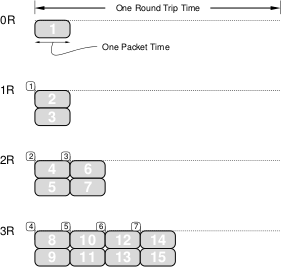
\includegraphics[width=0.48\textwidth]{img/slowstart}
  \end{center}
  \caption{The Chronology of a Slow-Start.\cite{Jacobson:1988:CAC:52325.52356}}
  \label{slowstart}
\end{wrapfigure}
is called \textit{slow start}. It is the responsible to gradually increase the amount of data that is in transit by observing that the a new package is injected into the network until the acknowledgment of a previous packages as arrives from the other end. In other words, it is used to avoid sending more data than the network is capable of transmit.\\

Slow start adds a variable window to the sender's TCP:  the congestion window, called ``\textit{cwnd}'' to the per-connection state.  When a new connection is established or restarting after a loss connection with a host, the congestion window is initialized to one segment, with the size of two times the maximum segment size (MMS)\footnote{The study of MMS is out of the scope of this paper, but more info could be found in \cite{rfc879} and \cite{rfc2460}} .  Each time an ACK is received, the congestion window is increased by one segment (1 MMS).  The sender can transmit up to the minimum of the congestion window and the advertised window.  The congestion window is flow control imposed by the sender, while the advertised window is flow control imposed by the receiver.  The former is based on the sender's assessment of perceived network congestion; the latter is related to the amount of available buffer space at the receiver for this connection.\\

The sender starts by transmitting one segment and waiting for its ACK. When that ACK is received, the congestion window is incremented from one to two, and two segments can be sent.  When each of those two segments is acknowledged, the congestion window is increased to four as seen in figure \ref{slowstart}. Here, the gray numbered boxes are packages and the white are the corresponding ACK. As each ACK arrives, two packages are generated, one for the ACK package that left the ``\textit{pipe}'' and one because an ACK opens the congestion window by one. This provides an exponential growth, it takes time \textbf{$Rlog_2 W$}\cite{Jacobson:1988:CAC:52325.52356}, where R is the round trip time and W is the window size. Although it is not exactly exponential because the receiver may delay its ACKs,typically sending one ACK for every two segments that it receives.\\

At some point the capacity of the internet can be reached, and an intermediate router will start discarding packets.  This tells the sender that its congestion window has gotten too large. Early implementations performed slow start only if the other end was on a different network.  Current implementations always perform slow start.\\


\subsubsection{The Congestion Avoidance Algorithm \cite{rfc2309}\cite{rfc2581}}
\indent In the ``\textit{slow start}" phase, if a when a lost occurs, half of the current window is saved as a Gresham a variable that is
 used to determine whether the slow start or congestion avoidance algorithm is used to control data transmission. After this, the \textit{cwnd} is set again to 1 and start to grown until it reaches the ssthresh again. Now, TCP goes into congestion avoidance mode, where for each ACK increases the cwnd in 1/cwnd. A congestion can occur when data arrives at a router whose output capacity is less than the sum of the inputs.  Congestion avoidance is a way to deal with lost packets.\\
	
This algorithm makes a fundamental assumption: \textit{the packet loss caused by damage is very small (much less than 1\%), therefore the loss of a packet signals congestion somewhere in the network between the source and destination}.  Two are the indication of package lost: a timeout occurring and the receipt of duplicate ACKs.\\

A good congestion avoidance strategy, must have two components: 1.- The endpoints should know when a congestion is about to occur or occurring into the network, and 2.- If a signal that alert the congestion is received, the network's utilization must decrease and increases if the signal isn't received.\\

When a networks is getting congested, the queue lengths will start to increase exponentially (because of slow-start). The system will collapse if the network doesn't throttle back the traffic sources at leas as quick as the queues are growing. The way that the network announces via dropped packets when demand is excessive, but says nothing if a connection is using less than its fair share. This is also another problem because causes underbuffering, also causing that the resources are not fully under full use.\\

The implementation of congestion avoidance is as simple as slow start, but with a slight difference\cite{Jacobson:1988:CAC:52325.52356}. The steps are:
\begin{enumerate}
\item On any timeout, set \textit{cwnd} to half the current window size. This produces a multiplicative decrease.
\item On each ack for new data, increase \textit{cwnd} by 1/\textit{cwnd}. Now cwnd has an additive increment so now the growth becomes linear.
\item When sending, send the minimum of the receiver's advertised window and \textit{cwnd}.
\end{enumerate}

A window of size cwnd packets will generate at most cwnd ACKs in one round trip time. Thus an increment of 1/cwnd per ACK will increase the window by at most one packet in one RTT. In TCP, windows and packet are in bytes so the increment translates to segsize*segsize/cwnd, where segsize is the segment size and cwnd is maintained in bytes.\\

Congestion avoidance and slow start are independent algorithms with different objectives.  But when congestion occurs TCP must slow down  its transmission rate of packets into the network, and then invoke slow start to get things going again. In practice they are implemented together. So, if cwnd is less than or equal to ssthresh, TCP is in slow start; otherwise TCP is performing congestion avoidance. Slow start continues until TCP is halfway to where it was when congestion occurred (since it recorded half of the window size that caused the problem ), and then congestion avoidance takes over.\\


\subsubsection{The Router's Congestion Avodance Complements}
After the ``congestion collapse" and with the growth in the last few decades of
 \begin{wrapfigure}{l}{0.5\textwidth}
  \begin{center}
    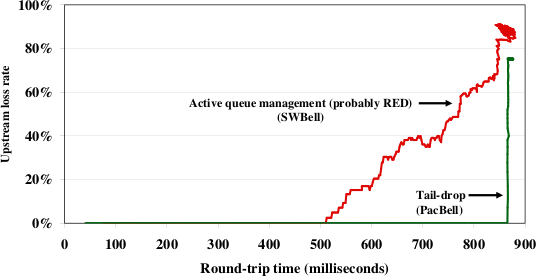
\includegraphics[width=0.48\textwidth]{img/overflows}
  \end{center}
  \caption{How Tail-drop management and RED AQM overflows\cite{Dischinger2007CRB}}
  \label{tdredof}
\end{wrapfigure}

Internet, it has become clear that the TCP congestion avoidance mechanisms,
while necessary and powerful, are not enough to provide a fully safe service,
and the control that can be accomplished from the edges of the networks has
proof that has a limit. So, in order to obtain a good service in all
circumstances, some mechanisms in the routers to complement this endpoint
congestion avoidance mechanisms are needed.\\

Two classes of router algorithms related with congestion avoidance control can
be distinguished: ``queue management" and ``scheduling" algorithms. While the
first one manage the length of packet queues by dropping packets when necessary
or appropriate, the second one determine which packet to send next, and are used
to manage the allocation of bandwidth among flows. It is important to notice
that while this two mechanisms are closely related, the performance that they
address are rather different and should be seen as complementary, and not as
replacements for each other.\\



\begin{enumerate}
\item \textbf{Managing the Routers Queue:} As we have seen in previous section, the traditional way to manage router queue
is, after set a maximum length for the queue, accept packages until this length
is reached, and then drop subsequent packages until a packet from the stack as
been transmitted. This technique is called ``tail drop", and has served the
Internet well enough for years, but it has two important drawbacks:\\

\begin{itemize}
\item It allows, in some situations, a single or few flows to monopolize the
queue space, preventing other connections from getting room in the queue.
\item The signaling is produced only when the queue is full, so it allows queue
to maintain almost full status for long periods.
\end{itemize}

If queue is full or almost full, an arriving burst will cause multiple packets to
be dropped, an this behavior can produce a global synchronization of flows
throttling back followed by sustained period of lowered link utilization, which
will impact in a reduce of overall throughput, and if a long flows arrives in
that period, the lock-out of the queue.\\

Besides tail drop, another two techniques can be applied in these situations.
The ``random drop on full" will produce that the router drops a randomly selected
packet from the full queue, which requires an $O(N)$ walk through the queue, when a
new packet arrives. Under the ``drop front on full", the router drops the packet
at the front of the queue. Either of these solve the lock-out problem, but
neither solves the full-queue.\\

\item \textbf{Active Queue Management and Random Early Detection} In the current Internet, dropped packets are used as a critical mechanism to
notify a end node when a congestion is presented. So, if a router is capable to
drop packets before the queue is full, and the end nodes take actions before the
buffers overflow, the full-queue problem is solved. This proactive approach is
know as ``active queue management" (AQM) and allows routers to control when and how
many packets to drop before buffers overflow.\\

For responsive flows, AQM can provide:
\begin{itemize}
\item reduce number of packets dropped in routers
\item provide lower-delay interactive service
\item avoid lock-out behavior
\end{itemize}

One AQM algorithm for routers is called ``Random Early Detection" or RED. The
algorithm drops arriving packets probabilistically, which increases as the
estimated average queue size grows, so it approach is based on the ``recent
past" events.\\

The RED algorithm consists of two main parts:

\begin{itemize}
\item Estimation of the average queue size
\item Packet drop decision
\end{itemize}

RED's particular algorithm for dropping is the culprit in the performance
improvement. 

\end{enumerate}

\subsection{Latency}
% 2.- Latency: When a new package arrives, it has to wait to the full queue get processed before its time, this way the package spent extra time waiting in the queue.
The latency a packet experiences in a network is made up of transmission
delay (the time it takes to send it across communications links), processing
delay (the time each network element spends handling the packet) and queuing
delay (the time spent waiting to be processed or retransmitted). But large
buffers only increase latency, and this only causes conflict with the needs
of nowadays applications.

Once packets in-fly reach a bottleneck, they begin to pool. Because the
characteristics already explained, more and more packets are coming, and this
queue continues to increase, which leads that each new arriving packet spending
more time in the queue than the predecessor packet, which means an
increase in the latency. Eventually, packets start to be dropped,
notifying the hosts of the presence of congestion on the path.

As stated in \cite{Dischinger2007CRB}, it is quite common to find these high-
latency queues in the last mile. The causes can be many, but among the most
common are both link quality at homes, as different implementations of traffic
shaping methods implemented by ISPs, or massive buffers set by the latter to
avoid loss of data, which can add a delay of up to several milliseconds.
Bottlenecks at the Internet's edge can easily move between the wireless
access (when its bandwidth is slow) and the provider's up-link, both of which
can have highly variable bandwidths.

For networks that use coaxial cable, multiple clients concatenated their
upward flows in a single transmission, resulting in a burst with a large
volume of data, which can led to a high fluctuation in latency. This
concatenation can also generate jitter time, which can be produce a miss
interpretation for some protocols of incipient congestion and cause to enter
into congestion control avoidance too early. The other type of highly used
networks are the DSL, which the more distance is between the supplier reduces
its transmission rate. That is why it is needed advanced signal processing and
error correction algorithms which can lead to high packet propagation delays.


%end section Fundation
%section Characterization
\section{Characterization of Bufferbloat}

\subsection{Backbone Routers}

As we already know, all internet routers contains buffers to hold packets during times of congestion. A widely used rule-of-thumb states that each link need a buffer of size $B = \overline{RTT} x C $, where $\overline{RTT}$ is the average round trip time of a flow passing across the link, and C is the data rate of the link. The main characteristic of bufferbloat is the existence of excessively large and frequently full buffers inside the network. Large buffers have been inserted all over the Internet without sufficient thought or testing, so router buffers are the single biggest contributor to uncertainty in the Internet.\\

The rule-of-thumb come from a desire to keep the link as busy as possible so, the throughput of the network is always as big as possible. But, because the way that TCP works, no matter how big the buffer is at the bottleneck link, TCP will cause the buffer to overflow.\\ 

Overbuffering is a bad idea for two reasons:
\begin{enumerate}
\item It complicates the design of high-speed routers, leading to higher power consumption, more board space, and lower density.
\item It increases end-to-end delay in the presence of congestion
\end{enumerate}

As seen in 2.2, large buffers only increases latency, and this only causes conflict with the needs of real time applications.\\

The most important fact of sizing a buffer is to make that sure that while the sender pauses, the router buffer doesn't go empty and force the bottleneck to go idle. Again, the idea is to keep as much throughput as possible so the use of the link is fully utilized. The buffer will avoid to idle if the first packet from the sender shows up at the buffer just as it hits empty. In previous section, we define that after a lost is detected, the cwnd is set to half of is last value, so if we denote as $(W_{max} /2)/C$ the amount of time that packets are sent in congestion phase, and as $B/C$ the time that takes a buffer with size B to drain, the size of a buffer B needed is $B \leq (W_{max} /2)$.\\

Also from \cite{main:ref:1}, we can see that the rule-of-thumb doesn't longer apply to backbone routers, and a better estimator of the size of a buffer with n flows would be no more than $B = (\overline{RTT}xC)/\sqrt{n}$. With the assumption that short-flows plays a very small effect, and that the buffer size is dictated by the number of long flows, this factor will be proof that routers are much longer than they need to be, possible by two order of magnitude.


\subsection{Residential BroadBand Networks}
It is well know that residential networks are often the bottleneck in the last
mile access to the Internet Infrastructure. This could be because the ISP's of
both of the most popular ways to access (DSL and cable networks) to internet
today, use traffic shaping methods and ,as seen in previous sections, deploy
massive queues that can delay packets for several hundred milliseconds.\\

Both shares the asymmetric bandwidths; they downstream bandwidth is higher than
their upstream bandwidth, but in cable networks a single coaxial cable shares
multiple customers, they can concatenate multiple upstream packets into a single
transmission, which result in short bursts at high data rates, so the latency
can heavily fluctuate. This concatenation can produce a jitter time, that under
high network load can be higher than end-to-end jitter over the entire path
under normal load, which can be produce a miss interpretation for some protocols
of incipient congestion and cause to enter into congestion control avoidance too
early.\\

In the other hand, in DSL networks, the maximum data transmission
rate falls with increasing distance from the head, thus in order to boost the
transmission rate, DSL relies on advanced signal processing and error correction
algorithms which can lead to high packet propagation delays .\\




%end section Characterization

%%%%%%%%%%%%%%%%%%%%%%%%%%%
%incluyo referencias
\bibliography{references,rfc}{}
%%%%%%%%%%%%%%%%%%%%%%%%%%%%

\end{document}
